\documentclass{beamer}
\usepackage[utf8]{inputenc}

\usetheme{Madrid}
\usecolortheme{default}
\useinnertheme{circles}

\definecolor{Logo1}{rgb}{0.208, 0.2865, 0.373}
\definecolor{Logo2}{rgb}{0.000, 0.674, 0.863}

\setbeamercolor*{palette primary}{bg=Logo1, fg=white}
\setbeamercolor*{palette secondary}{bg=Logo2, fg=white}
\setbeamercolor*{palette tertiary}{bg=white, fg=Logo1}
\setbeamercolor*{palette quaternary}{bg=Logo1,fg=white}
\setbeamercolor{structure}{fg=Logo1} % itemize, enumerate, etc
\setbeamercolor{section in toc}{fg=Logo1} % TOC sections

\usepackage{graphicx,animate}
%------------------------------------------------------------
%This block of code defines the information to appear in the
%Title page
\title[Linear Algebra] %optional
{Column Space \& Nullspace; Solving Ax=0 \& Ax=b}

\subtitle{Lecture 3}

\author[11910803@mail.sustech.edu.cn] % (optional)
{
    Zhang Ce
}

\institute[] % (optional)
{
    Department of Electrical and Electronic Engineering\\
    Southern University of Science and Technology
}

\date[2021.10.12] % (optional)
{2021.10.12}


%End of title page configuration block
%------------------------------------------------------------



%------------------------------------------------------------
%The next block of commands puts the table of contents at the
%beginning of each section and highlights the current section:

\AtBeginSection[]
{
\begin{frame}
    \frametitle{Table of Contents}
    \tableofcontents[currentsection]
\end{frame}
}
%------------------------------------------------------------


\begin{document}

%The next statement creates the title page.
\frame{\titlepage}


%---------------------------------------------------------
%This block of code is for the table of contents after
%the title page
\begin{frame}
\frametitle{Table of Contents}
\tableofcontents
\end{frame}
%---------------------------------------------------------
\section{A Brief Review of Last Lecture}
\begin{frame}{Last Lecture, We Discuss\dots}
Three parts in last lecture:
    \begin{enumerate}
        \item Row Exchanges and $PA=LU$ Factorization\\
        permutation matrix, process of $PA=LU$ factorization
        \item Inverse of Matrix\\
        existence of inverse, calculation of inverse, block inverse
        \item Vector Spaces and Subspaces\\
        definition of vector spaces and subspaces
    \end{enumerate}

Don't forget row method and column method for matrix multiplication. Things will get easier if you know these methods!
\end{frame}

\begin{frame}{Matrix Multiplication}
\begin{examples}
Compute the matrix multiplication.
    \begin{equation*}
        \left[ \begin{matrix}
            3&		-1&       1\\
            1&		 0&       1\\
            0&		 1&       2\\
        \end{matrix} \right] \left[ \begin{matrix}
            1&		 0&       1\\
            1&		-1&      -1\\
            1&		 2&       1\\
        \end{matrix} \right] =\left[ \begin{matrix}
            3&		 3&       5\\
            2&		 2&       2\\
            3&		 3&       1\\
        \end{matrix} \right]
    \end{equation*}
\end{examples}

\begin{enumerate}
    \item The regular (row-col) way. (Row of A) multiply (Column of B).
    \item The row way. Linear combination of (Row of B).
    \item The column way. Linear combination of (Column of A).
    \item The col-row way. (Column of A) multiply (Row of B).
\end{enumerate}

There is also an additional method: block method.
\end{frame}

\begin{frame}{Why $P^T=P^{-1}$?}
Why $P^T=P^{-1}$? A direct explanation:
\vspace{3pt}

\begin{columns}
\column{0.5\textwidth}
\begin{equation*}
    P=\left[ \begin{matrix}
        0&		1&		0&		0\\
        0&		0&		1&		0\\
        0&		0&		0&		1\\
        1&		0&		0&		0\\
    \end{matrix} \right]
\end{equation*}

\begin{itemize}
    \item 1 at $(1,2)$: (Row 2) $\rightarrow$ (Row 1).
    \item 1 at $(2,3)$: (Row 3) $\rightarrow$ (Row 2).
    \item 1 at $(3,4)$: (Row 4) $\rightarrow$ (Row 3).
    \item 1 at $(4,1)$: (Row 1) $\rightarrow$ (Row 4).
\end{itemize}

\column{0.5\textwidth}
\begin{equation*}
    P^T=\left[ \begin{matrix}
        0&		0&		0&		1\\
        1&		0&		0&		0\\
        0&		1&		0&		0\\
        0&		0&		1&		0\\
    \end{matrix} \right]
\end{equation*}

\begin{itemize}
    \item 1 at $(2,1)$: (Row 1) $\rightarrow$ (Row 2).
    \item 1 at $(3,2)$: (Row 2) $\rightarrow$ (Row 3).
    \item 1 at $(4,3)$: (Row 3) $\rightarrow$ (Row 4).
    \item 1 at $(1,4)$: (Row 4) $\rightarrow$ (Row 1).
\end{itemize}
\end{columns}

\vspace{7pt}
Exchange A and B then exchange B and A will result in exchange nothing.

\end{frame}

\begin{frame}{Existence of Inverse}
According to definition, if it has an inverse, there exist a matrix $B$ to let $AB=I$, thus, $B$ is the inverse of $A$.
\begin{equation*}
    \left[ \begin{matrix}
        1&		2\\
        3&		6\\
    \end{matrix} \right] \left[ \begin{matrix}
        x&		\cdot\\
        y&		\cdot\\
    \end{matrix} \right] =\left[ \begin{matrix}
        1&		0\\
        0&		1\\
    \end{matrix} \right]
\end{equation*}

Recall the column method of matrix multiplication:
\begin{equation*}
    x\left[ \begin{array}{c}
        1\\
        3\\
    \end{array} \right] +y\left[ \begin{array}{c}
        2\\
        6\\
    \end{array} \right] =\left[ \begin{array}{c}
        1\\
        0\\
    \end{array} \right]
\end{equation*}

It may lead you to think about column picture.

\vspace{3pt}
Linear combinations of the 2 column vectors are still on the straight line.

\vspace{3pt}
Therefore, the inverse cannot exist for this matrix $A$.

\vspace{3pt}
How about multiplying this matrix on the left side?
\end{frame}

\begin{frame}{Gauss-Jordan Method: Another Way}
\begin{example}
    Find the inverse of the following matrix:
    \begin{equation*}
        A=\left[ \begin{matrix}
            1&		2\\
            3&		7\\
        \end{matrix} \right]
    \end{equation*}
\end{example}

\textbf{Solution:}

Remember: Always do row operations.
\begin{equation*}
    \left[ \begin{matrix}
        1&		2&		1&		0\\
        3&		7&		0&		1\\
    \end{matrix} \right] \rightarrow \left[ \begin{matrix}
        1&		2&		1&		0\\
        0&		1&		-3&		1\\
    \end{matrix} \right] \rightarrow \left[ \begin{matrix}
        1&		0&		7&		-2\\
        0&		1&		-3&		1\\
    \end{matrix} \right]
\end{equation*}

Or... Column operations!
\begin{equation*}
    \left[ \begin{matrix}
        1&		2\\
        3&		7\\
        1&		0\\
        0&		1\\
    \end{matrix} \right] \rightarrow \left[ \begin{matrix}
        1&		0\\
        3&		1\\
        1&		-2\\
        0&		1\\
    \end{matrix} \right] \rightarrow \left[ \begin{matrix}
        1&		0\\
        0&		1\\
        7&		-2\\
        -3&		1\\
    \end{matrix} \right]
\end{equation*}
\end{frame}



\begin{frame}{Block Method to Find the Inverse}
\begin{example}
    Find the inverse of this matrix, given that $A,B,C$ are all invertible matrices. Please express the result in matrix form.
    \begin{equation*}
        L=\left[ \begin{matrix}
            A&		0\\
            B&		C\\
        \end{matrix} \right]
    \end{equation*}
\end{example}

\textbf{Solution:}

Core idea: Treat all block matrices as a single entry.
\begin{equation*}
    \left[ \begin{matrix}
        A&		0&		I&		0\\
        B&		C&		0&		I\\
    \end{matrix} \right] \rightarrow \left[ \begin{matrix}
        A&		0&		I&		0\\
        0&		C&		-BA^{-1}&		I\\
    \end{matrix} \right] \rightarrow \left[ \begin{matrix}
        I&		0&		A^{-1}&		0\\
        0&		I&		-C^{-1}BA^{-1}&		C^{-1}\\
    \end{matrix} \right]
\end{equation*}

\begin{equation*}
    L^{-1}=\left[ \begin{matrix}
        A^{-1}&		0\\
        -C^{-1}BA^{-1}&		C^{-1}\\
    \end{matrix} \right]
\end{equation*}

A good question to ask: why not right-multiply $C^{-1}$ in the final step?
\end{frame}

\section{Vector Spaces and Subspaces}
\begin{frame}{Vectors vs Points}
When we describe a vector, we always use arrows. But, when we describe multiple vectors, treat it as points! That is a very important concept in linear algebra.

\vspace{3pt}
Hope this video can help you establish this concept.

\vspace{8pt}

Source: The Essence of Linear Algebra -by \emph{3Blue1Brown} P3 04:44\\
\vspace{3pt}
\url{https://www.bilibili.com/video/BV1ys411472E?p=3}

\vspace{8pt}

In linear algebra, lines, planes, spaces can all be treated as a collection of vectors. That is why they are called vector spaces!

\vspace{3pt}
By the way, this series of video is really useful and can help you get a deeper understanding in linear algebra, I recommend all of you spend some time watching the first few sections after class.

\end{frame}


\begin{frame}{Subspaces of $\mathbb{R} ^2$}
Now, thing will be easier to understand the definition of vector spaces and subspaces.

\vspace{3pt}
According to definiton, a vector space inside $\mathbb{R} ^2$ is a subspace of $\mathbb{R} ^2$.

\vspace{3pt}
Try to decide whether the following ones are subspaces of $\mathbb{R} ^2$?

\begin{enumerate}
    \item $S_1=\left\{ \left( x,0 \right) |\: x\in \mathbb{R} \right\}$
    \item $S_2=\left\{ \left( x,y \right) |\: 4x+y=0 \:\&\: x,y\in \mathbb{R} \right\}$
    \item $S_3=\left\{ \left( x,y \right) |\: x+y=1 \:\&\: x,y\in \mathbb{R} \right\}$
    \item $S_4=\left\{ \left( x,y \right) |\: xy=0 \:\&\: x,y\in \mathbb{R} \right\}$\
    \item $S_5=S_1\cup S_2$
    \item $S_6=S_1\cap S_2$
    \item $S_7=\mathbb{R} ^2$
\end{enumerate}

\vspace{3pt}
A conclusion: the intersection of 2 subspaces is still a subspace, but smaller. Can you find the reason? (Use the definition to verify.)

\vspace{3pt}
Now, try to list all the subspaces for $\mathbb{R} ^2$\dots
\end{frame}

\begin{frame}{Subspaces of $\mathbb{R} ^2$}
Subspaces of $\mathbb{R} ^2$ (3 types):
\begin{enumerate}
    \item The origin. That is the zero vector $\left[ \begin{array}{c}
        0\\
        0\\
    \end{array} \right] $.
    \item Straight lines across the origin.
    \vspace{7pt}
    \item  $\mathbb{R} ^2$ itself.
\end{enumerate}

\vspace{5pt}
Can I say $\mathbb{R} ^1$? Why?

\vspace{3pt}
The vectors stored in $\mathbb{R} ^1$ have only 1 component, while the vectors in $\mathbb{R} ^2$ have 2. I have to say they are quite similar because they are both lines, but they are not the same.

\vspace{3pt}
Try to list the subspaces of $\mathbb{R} ^5$.
\end{frame}

\section{Column Space and Nullspace}
\begin{frame}{Vector Spaces Defined from a Matrix}
Given a matrix $A$:
\begin{equation*}
    \left[ \begin{matrix}
        1&		1\\
        1&		2\\
        3&		1\\
    \end{matrix} \right]
\end{equation*}

Naturally, this matrix has 2 column vectors already:
\begin{equation*}
    \left[ \begin{array}{c}
        1\\
        1\\
        3\\
    \end{array} \right] ,\: \left[ \begin{array}{c}
        1\\
        2\\
        1\\
    \end{array} \right]
\end{equation*}

Now, find a vector space contains these 2 vectors. It is a subspace of $\mathbb{R} ^3$.

\vspace{3pt}
Which other vectors should exist in this subspace to satisfy the definition of vector spaces?

\vspace{3pt}

\end{frame}

\begin{frame}{Column Space}
To satisfy the definition of vector spaces, the scalar multiplications of those vectors (2 lines) and the addition of those vectors (the vectors between the lines) are in the final subspace. We can also say \alert{linear combinations} of the 2 vectors are in the final subspace.

\vspace{3pt}
Can you imagine the figure of this subspace? It is a 2-dimensional space across the origin in $\mathbb{R} ^3$ space. Make sure you understand it, important!
\begin{figure}
    \centering
    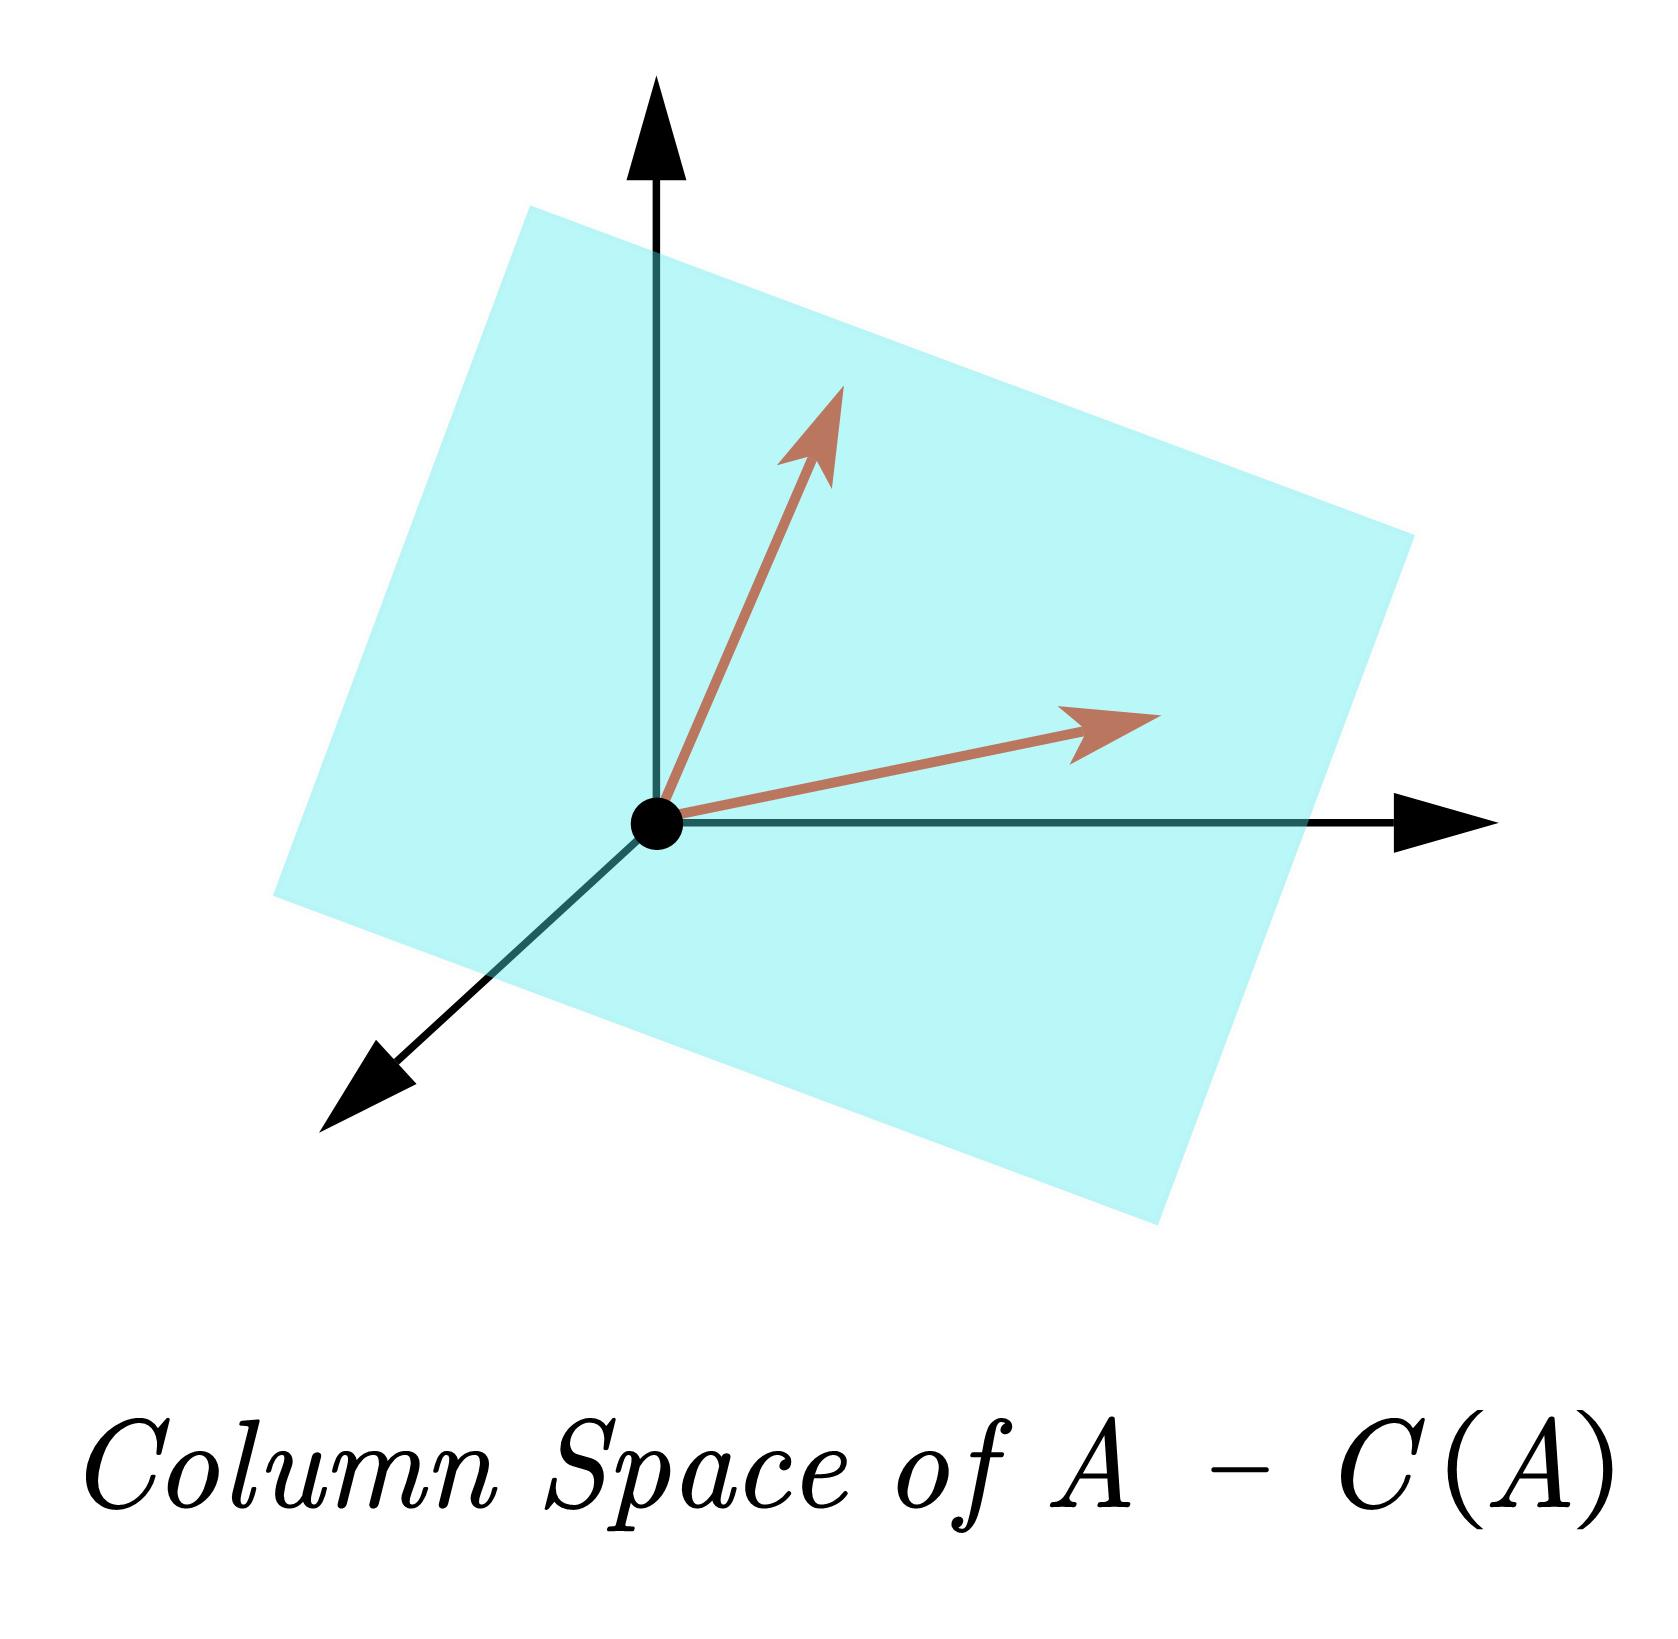
\includegraphics[width=0.3\textwidth]{column.jpg}
\end{figure}
\vspace{-14pt}
This special subspace is the column space of matrix $A$.

\vspace{3pt}
4 vectors in $\mathbb{R} ^9$ will form (or \alert{span})\dots
\end{frame}

\begin{frame}{Associate Column Space with Linear Equation}
\begin{equation*}
    A=\left[ \begin{matrix}
        1&		1&		2\\
        2&		1&		3\\
        4&		1&		5\\
        7&		1&		8\\
    \end{matrix} \right]
\end{equation*}

The column space of $A\:(4\times3)$ is a subspace of $\mathbb{R}^4$.

\vspace{3pt}
Can 3 column vectors in $A$ span the whole $\mathbb{R}^4$ space?

\vspace{3pt}
We have known that every matrix represent a system of linear equations. Think about the linear equation system corresponding to matrix $A$. How many equations? How many unknowns?
\begin{equation*}
    \left[ \begin{matrix}
        1&		1&		2\\
        2&		1&		3\\
        4&		1&		5\\
        7&		1&		8\\
    \end{matrix} \right] \left[ \begin{array}{c}
        x_1\\
        x_2\\
        x_3\\
    \end{array} \right] =\left[ \begin{array}{c}
        b_1\\
        b_2\\
        b_3\\
        b_4\\
    \end{array} \right]
\end{equation*}
Can this equation system always have a solution?
\end{frame}

\begin{frame}{Associate Column Space with Linear Equation}
\begin{equation*}
    \left[ \begin{matrix}
        1&		1&		2\\
        2&		1&		3\\
        4&		1&		5\\
        7&		1&		8\\
    \end{matrix} \right] \left[ \begin{array}{c}
        x_1\\
        x_2\\
        x_3\\
    \end{array} \right] =\left[ \begin{array}{c}
        b_1\\
        b_2\\
        b_3\\
        b_4\\
    \end{array} \right]
\end{equation*}

4 equations, 3 unknowns, usually make the equation system not solvable.

\vspace{3pt}
Think row picture of this linear equation system. Each row represent a plane in $\mathbb{R}^3$ space, the solution is the intersection of 4 planes.

\vspace{3pt}
An important question is which $b$s allow this equation system to have solutions?

\vspace{3pt}
Give me some right-hand side $b$ to make the equation system solvable.

\vspace{-7pt}
\begin{columns}
    \column{0.5\textwidth}
    \begin{equation*}
        \left[ \begin{matrix}
            1&		1&		2\\
            2&		1&		3\\
            4&		1&		5\\
            7&		1&		8\\
        \end{matrix} \right] \left[ \begin{array}{c}
            x_1\\
            x_2\\
            x_3\\
        \end{array} \right] =\left[ \begin{array}{c}
            0\\
            0\\
            0\\
            0\\
        \end{array} \right]
    \end{equation*}

    \column{0.5\textwidth}
    \begin{equation*}
        \left[ \begin{matrix}
            1&		1&		2\\
            2&		1&		3\\
            4&		1&		5\\
            7&		1&		8\\
        \end{matrix} \right] \left[ \begin{array}{c}
            x_1\\
            x_2\\
            x_3\\
        \end{array} \right] =\left[ \begin{array}{c}
            1\\
            2\\
            4\\
            7\\
        \end{array} \right]
    \end{equation*}
    \end{columns}
\end{frame}

\begin{frame}{Associate Column Space with Linear Equation}
How about we write the solutions first, find which $b$ lead to this solution?
\begin{equation*}
    \left[ \begin{matrix}
        1&		1&		2\\
        2&		1&		3\\
        4&		1&		5\\
        7&		1&		8\\
    \end{matrix} \right] \left[ \begin{array}{c}
        x_1\\
        x_2\\
        x_3\\
    \end{array} \right] =\left[ \begin{array}{c}
        b_1\\
        b_2\\
        b_3\\
        b_4\\
    \end{array} \right]
\end{equation*}

The left side gives all possible linear combinations of the 3 column vectors.

\vspace{3pt}
You may already discover, the equation system is solvable exactly when $b$ is in $C(A)$.

\vspace{3pt}
Are these 3 column vectors \alert{linearly independent}? Or, do they all contribute to expand the dimension of column space?

\vspace{3pt}
No, because even if we delete a column, the column space will not change. We will call the linearly independent columns (contribute to column space) that come first pivot columns later.
\end{frame}

\begin{frame}{Nullspace}
Nullspace contains all the solutions $x=\left[ \begin{array}{c}
        x_1\\
        x_2\\
        x_3\\
    \end{array} \right]$
to
\begin{equation*}
    \left[ \begin{matrix}
        1&		1&		2\\
        2&		1&		3\\
        4&		1&		5\\
        7&		1&		8\\
    \end{matrix} \right] \left[ \begin{array}{c}
        x_1\\
        x_2\\
        x_3\\
    \end{array} \right] =\left[ \begin{array}{c}
        0\\
        0\\
        0\\
        0\\
    \end{array} \right]
\end{equation*}

Give me some obvious solutions.

\vspace{-3pt}
\begin{columns}
    \column{0.5\textwidth}
    \begin{equation*}
        \left[ \begin{matrix}
            1&		1&		2\\
            2&		1&		3\\
            4&		1&		5\\
            7&		1&		8\\
        \end{matrix} \right] \left[ \begin{array}{c}
            0\\
            0\\
            0\\
        \end{array} \right] =\left[ \begin{array}{c}
            0\\
            0\\
            0\\
            0\\
        \end{array} \right]
    \end{equation*}

    \column{0.5\textwidth}
    \begin{equation*}
        \left[ \begin{matrix}
            1&		1&		2\\
            2&		1&		3\\
            4&		1&		5\\
            7&		1&		8\\
        \end{matrix} \right] \left[ \begin{array}{c}
            1\\
            1\\
            -1\\
        \end{array} \right] =\left[ \begin{array}{c}
            0\\
            0\\
            0\\
            0\\
        \end{array} \right]
    \end{equation*}
\end{columns}
\end{frame}

\begin{frame}{Nullspace}
Well, you can write a complete solution to this equation system by observation. (I don't want to spend time proving that.)

\begin{equation*}
    \left[ \begin{matrix}
        1&		1&		2\\
        2&		1&		3\\
        4&		1&		5\\
        7&		1&		8\\
    \end{matrix} \right] \left[ \begin{array}{c}
        c\\
        c\\
        -c\\
    \end{array} \right] =\left[ \begin{array}{c}
        0\\
        0\\
        0\\
        0\\
    \end{array} \right]
\end{equation*}

where $c$ is a constant.

\vspace{3pt}
So the nullspace looks like\dots \:A straight line across the origin!

\begin{figure}
    \centering
    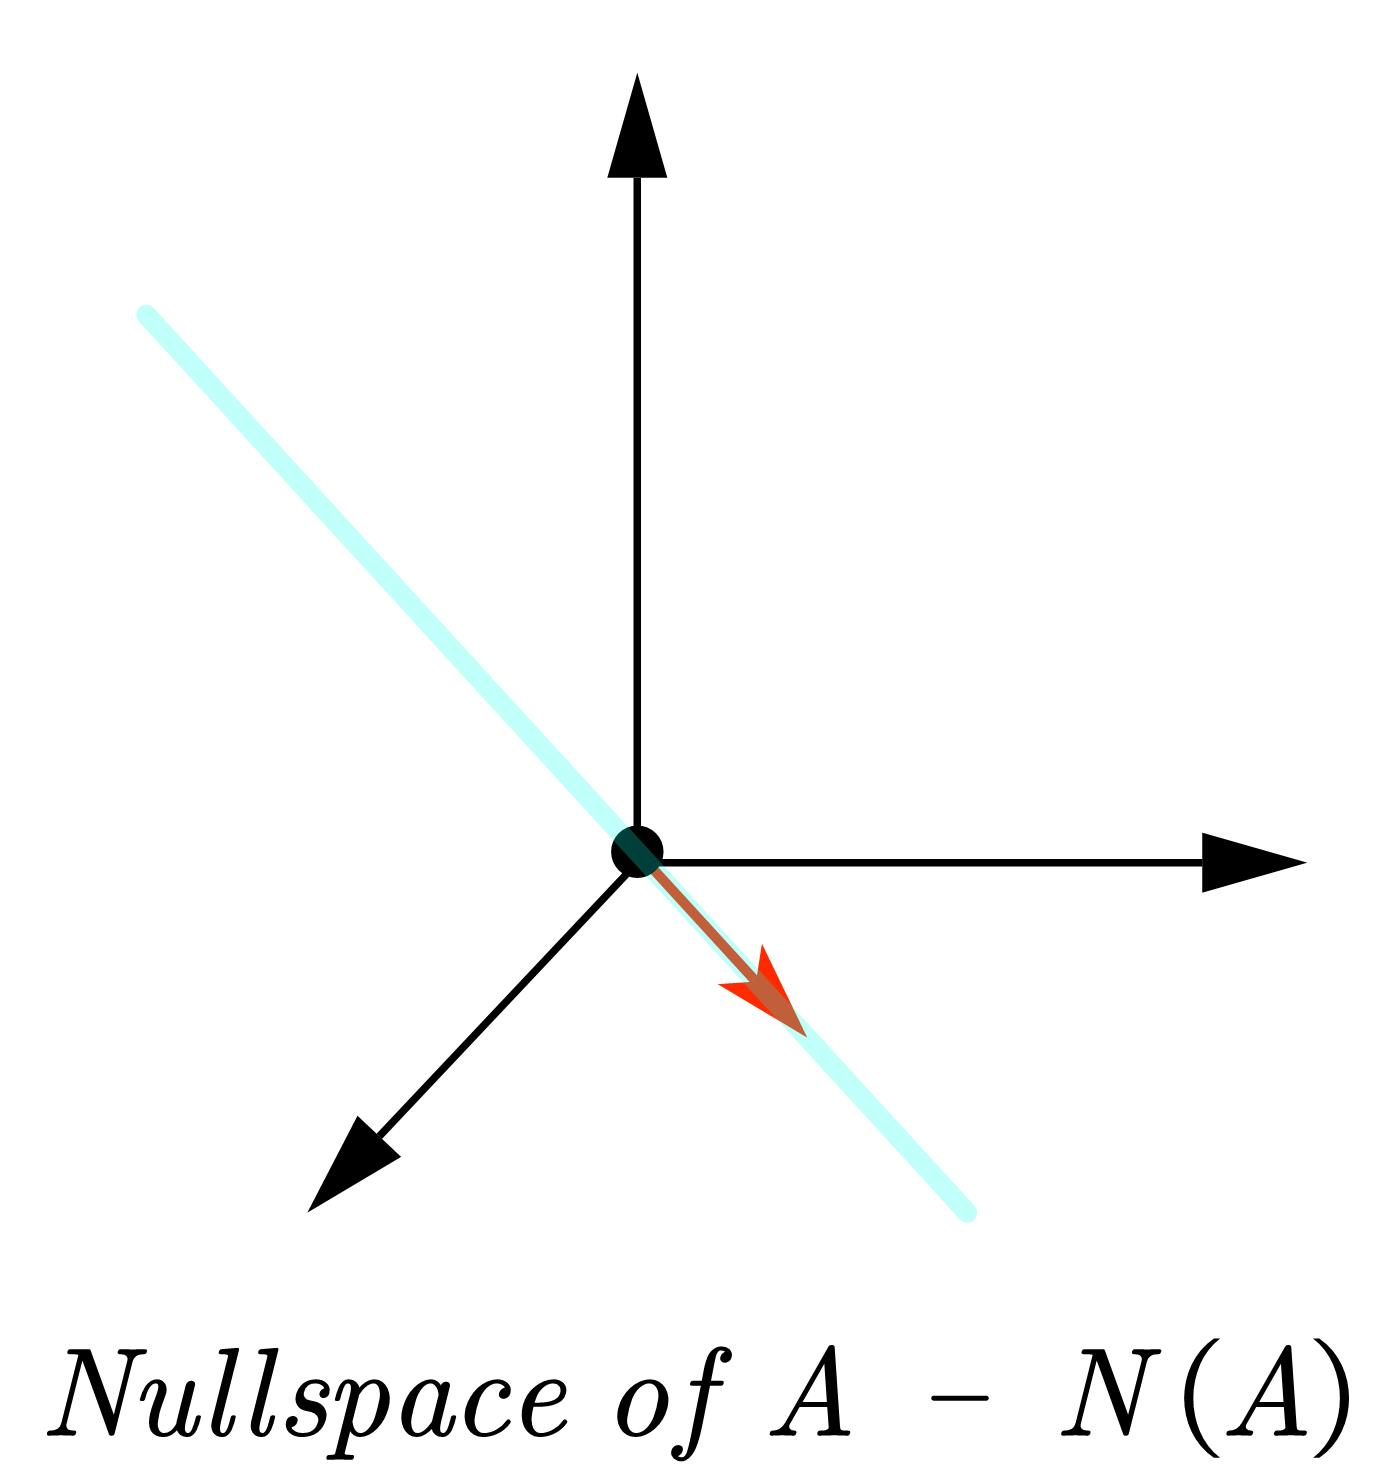
\includegraphics[width=0.25\textwidth]{null.jpg}
\end{figure}
\end{frame}

\begin{frame}{Nullspace}
A straight line across the origin\dots Is it a subspace of $\mathbb{R}^3$?

\vspace{3pt}
Yes, it is. Are all the nullspaces subspaces? How to illustrate that?

\begin{itemize}
    \item Firstly, let's verify addition. We choose 2 vectors $u,v$ in the nullspace, they satisfy $Au=Av=0$. The addition vector $u+v$ is still in the nullspace since $A(u+v)=0$.
    \item Secondly, let's verify scalar multiplication. We have a vector $v$ in the nullspace, which gives us $Av=0$. The vector $cv$ is still in the nullspace since $A(cv)=0$.
\end{itemize}

The nullspace of $A\:(4\times3)$ is a subspace of $\mathbb{R}^3$.

\vspace{3pt}
Is the solutions still a subspace when the right-hand side $b$ not equals to zero? Definitely no, because zero vector isn't in the solution space.

\vspace{3pt}
Now, you have known 2 important subspaces defined by a matrix. At the end of this chapter, you will know 4 subspaces. We are now approaching the core of linear algebra.

\end{frame}

\section{Solving Ax=0}
\begin{frame}{Introduction}
This section introduces an algorithm, it will take up approximately 20 marks in your midterm exam.

\vspace{3pt}
A good example question is important to make you understand the solving process. In this part, let's look at this matrix.

\begin{equation*}
    A=\left[ \begin{matrix}
        1&		3&		3&		3\\
        2&		6&		8&		10\\
        3&		9&		11&		13\\
    \end{matrix} \right]
\end{equation*}

The question is how to find the solution of $Ax=0$. In this example, $x$ has 4 components.

\vspace{3pt}
We have learnt an algorithm for solving linear equation systems - Gauss Elimination. Gauss elimination can help us simplify the equations and find the pivots, and it will never change the nullspace.
\end{frame}

\begin{frame}{Gauss Elimination}
Do Gauss elimination for matrix $A$.

\vspace{3pt}
The first step:
\begin{equation*}
    \left[ \begin{matrix}
        1&		3&		3&		3\\
        2&		6&		8&		10\\
        3&		9&		11&		13\\
    \end{matrix} \right] \rightarrow \left[ \begin{matrix}
        1&		3&		3&		3\\
        0&		0&		2&		4\\
        0&		0&		2&		4\\
    \end{matrix} \right]
\end{equation*}

It makes some difficulties for us\dots The second column has no pivots.

\vspace{3pt}
In Chapter 1 (square matrix cases), we call this situation permanent failure (or singular). But it doesn't mean $Ax=0$ has no nonzero solution.

\begin{equation*}
    \left[ \begin{matrix}
        1&		0&		0\\
        0&		0&		0\\
        0&		0&		0\\
    \end{matrix} \right] \left[ \begin{array}{c}
        x_1\\
        x_2\\
        x_3\\
    \end{array} \right] =\left[ \begin{array}{c}
        0\\
        0\\
        0\\
    \end{array} \right]
\end{equation*}

For the equation system above, $\left[ \begin{matrix}
	0&		1&		1\\
\end{matrix} \right] ^T$ is a solution. In Chapter 1, we avoid this case, but now we face it directly. My advice is: find the next pivot and go on.
\end{frame}

\begin{frame}{Gauss Elimination}
\begin{equation*}
    A=\left[ \begin{matrix}
        1&		3&		3&		3\\
        2&		6&		8&		10\\
        3&		9&		11&		13\\
    \end{matrix} \right] \rightarrow \left[ \begin{matrix}
        1&		3&		3&		3\\
        0&		0&		2&		4\\
        0&		0&		2&		4\\
    \end{matrix} \right] \rightarrow \left[ \begin{matrix}
        1&		3&		3&		3\\
        0&		0&		2&		4\\
        0&		0&		0&		0\\
    \end{matrix} \right] =U
\end{equation*}

Gauss elimination ends. The result is not a strict upper triangular matrix, we call it echelon form ($U$).

\vspace{3pt}
The matrix $A$ has 2 pivots, that is called the \alert{rank} of matrix $A$.
\begin{equation*}
    rank\,\,r\,\,=\,\,\# \,of\,\,pivots
\end{equation*}

During this elimination process which of the following are still unchanged?

\begin{itemize}
    \item Column Space
    \item Nullspace
    \item The subspace spanned by the rows. (Row Space)
\end{itemize}

So we simplify the equation system $Ax=0\Leftrightarrow Ux=0$.
\end{frame}

\begin{frame}{Pivot Columns and Free Columns}
The most important step different with Chapter 1 comes.

\vspace{3pt}
The simplified equation system becomes
\begin{equation*}
    \left[ \begin{matrix}
        1&		3&		3&		3\\
        0&		0&		2&		4\\
        0&		0&		0&		0\\
    \end{matrix} \right] \left[ \begin{array}{c}
        x_1\\
        x_2\\
        x_3\\
        x_4\\
    \end{array} \right] =\left[ \begin{array}{c}
        0\\
        0\\
        0\\
    \end{array} \right]
\end{equation*}

Find the pivots and they determine the pivot columns, the rest are free columns. In this example, column 1 \& 3 are pivot columns, column 2 \& 4 are free columns.

\vspace{3pt}
We can take any number for the coefficient of free columns and solve the coefficient for pivot columns by back-substitution. That is we can choose $x_2$ \& $x_4$ randomly.

\vspace{3pt}
Commonly, we choose to set a free column coefficient 1 and the others 0.
\end{frame}

\begin{frame}{Back-Substitution}
\begin{columns}
    \column{0.5\textwidth}
    \begin{equation*}
        \left[ \begin{matrix}
            1&		3&		3&		3\\
            0&		0&		2&		4\\
            0&		0&		0&		0\\
        \end{matrix} \right] \left[ \begin{array}{c}
            x_1\\
            1\\
            x_3\\
            0\\
        \end{array} \right] =\left[ \begin{array}{c}
            0\\
            0\\
            0\\
        \end{array} \right]
    \end{equation*}

    \column{0.5\textwidth}
    \begin{equation*}
        \left[ \begin{matrix}
            1&		3&		3&		3\\
            0&		0&		2&		4\\
            0&		0&		0&		0\\
        \end{matrix} \right] \left[ \begin{array}{c}
            x_1\\
            0\\
            x_3\\
            1\\
        \end{array} \right] =\left[ \begin{array}{c}
            0\\
            0\\
            0\\
        \end{array} \right]
    \end{equation*}
\end{columns}

\vspace{5pt}
Write their corresponding equation systems.
\begin{equation*}
    \begin{cases}
        x_1+3x_2+3x_3+3x_4=0\\
        \qquad\qquad\ \ \:           2x_3+4x_4=0\\
        \qquad\qquad\qquad\qquad\:\:                     0=0\\
    \end{cases}
\end{equation*}

Solve the coefficients of pivot columns by back-substitution now.

\vspace{-8pt}
\begin{columns}
    \column{0.5\textwidth}
    \begin{equation*}
        \left[ \begin{matrix}
            1&		3&		3&		3\\
            0&		0&		2&		4\\
            0&		0&		0&		0\\
        \end{matrix} \right] \left[ \begin{array}{c}
            -3\\
            1\\
            0\\
            0\\
        \end{array} \right] =\left[ \begin{array}{c}
            0\\
            0\\
            0\\
        \end{array} \right]
    \end{equation*}

    \column{0.5\textwidth}
    \begin{equation*}
        \left[ \begin{matrix}
            1&		3&		3&		3\\
            0&		0&		2&		4\\
            0&		0&		0&		0\\
        \end{matrix} \right] \left[ \begin{array}{c}
            3\\
            0\\
            -2\\
            1\\
        \end{array} \right] =\left[ \begin{array}{c}
            0\\
            0\\
            0\\
        \end{array} \right]
    \end{equation*}
\end{columns}

\end{frame}

\begin{frame}{Finally: Get the Solution}
These solutions can be called \alert{paticular solution}s.
\vspace{-5pt}
\begin{columns}
    \column{0.5\textwidth}
    \begin{equation*}
        \left[ \begin{matrix}
            1&		3&		3&		3\\
            0&		0&		2&		4\\
            0&		0&		0&		0\\
        \end{matrix} \right] \left[ \begin{array}{c}
            -3\\
            1\\
            0\\
            0\\
        \end{array} \right] =\left[ \begin{array}{c}
            0\\
            0\\
            0\\
        \end{array} \right]
    \end{equation*}

    \column{0.5\textwidth}
    \begin{equation*}
        \left[ \begin{matrix}
            1&		3&		3&		3\\
            0&		0&		2&		4\\
            0&		0&		0&		0\\
        \end{matrix} \right] \left[ \begin{array}{c}
            3\\
            0\\
            -2\\
            1\\
        \end{array} \right] =\left[ \begin{array}{c}
            0\\
            0\\
            0\\
        \end{array} \right]
    \end{equation*}
\end{columns}

\vspace{3pt}


We can take any number for the coefficient of free columns $x_2$ \& $x_4$.
\vspace{-5pt}
\begin{columns}
    \column{0.5\textwidth}
    \begin{equation*}
        \left[ \begin{matrix}
            1&		3&		3&		3\\
            0&		0&		2&		4\\
            0&		0&		0&		0\\
        \end{matrix} \right] \left[ \begin{array}{c}
            -3x_2\\
            x_2\\
            0\\
            0\\
        \end{array} \right] =\left[ \begin{array}{c}
            0\\
            0\\
            0\\
        \end{array} \right]
    \end{equation*}

    \column{0.5\textwidth}
    \begin{equation*}
        \left[ \begin{matrix}
            1&		3&		3&		3\\
            0&		0&		2&		4\\
            0&		0&		0&		0\\
        \end{matrix} \right] \left[ \begin{array}{c}
            3x_4\\
            0\\
            -2x_4\\
            x_4\\
        \end{array} \right] =\left[ \begin{array}{c}
            0\\
            0\\
            0\\
        \end{array} \right]
    \end{equation*}
\end{columns}

\vspace{3pt}
Add them, the solution is $x_2\left[ \begin{array}{c}
	-3\\
	1\\
	0\\
	0\\
\end{array} \right] +x_4\left[ \begin{array}{c}
	3\\
	0\\
	-2\\
	1\\
\end{array} \right]$. 2-dimensional space!
\end{frame}

\begin{frame}{Reduced Row Echelon Form (RREF)}
Recall in Chapter 1, we can do row operations to let the matrix become an identity matirx, then the solution appears on the right side. (That is how you find the inverse of matrix.)Similarly, we can have further simplication to this linear equation system.
\begin{equation*}
    U=\left[ \begin{matrix}
        1&		3&		3&		3\\
        0&		0&		2&		4\\
        0&		0&		0&		0\\
    \end{matrix} \right] \rightarrow \left[ \begin{matrix}
        1&		3&		0&		-3\\
        0&		0&		2&		4\\
        0&		0&		0&		0\\
    \end{matrix} \right] \rightarrow \left[ \begin{matrix}
        1&		3&		0&		-3\\
        0&		0&		1&		2\\
        0&		0&		0&		0\\
    \end{matrix} \right] =R
\end{equation*}

We only do row operations, $Ax=0\Leftrightarrow Ux=0\Leftrightarrow Rx=0$.

What we have done:
\begin{itemize}
    \item Eliminate entries on the top of pivots.
    \item Make the pivots all 1.
\end{itemize}

After this process, we have the Reduced Row Echelon Form (RREF) matrix $R$. Can you discover where the solutions appear?

\vspace{3pt}
Can you find the identity matrix in $R$?

\end{frame}

\begin{frame}{Reduced Row Echelon Form (RREF)}
Let's begin with the pivot columns:
\begin{equation*}
    \left[ \begin{matrix}
        {\color[RGB]{240, 0, 0} 1}&		{\color[RGB]{240, 0, 0} 0}&		{\color[RGB]{0, 128, 255} 3}&		{\color[RGB]{0, 128, 255} -3}\\
        {\color[RGB]{240, 0, 0} 0}&		{\color[RGB]{240, 0, 0} 1}&		{\color[RGB]{0, 128, 255} 0}&		{\color[RGB]{0, 128, 255} 2}\\
        0&		0&		0&		0\\
    \end{matrix} \right]
\end{equation*}

Generally, the RREF matrices are like
\begin{equation*}
    \left[ \begin{matrix}
        {\color[RGB]{240, 0, 0} I}&		{\color[RGB]{0, 128, 255} F}\\
        0&		0\\
    \end{matrix} \right]
\end{equation*}

I repeat the solution we have solved in previous slides. Correspondingly, I write the pivot column coefficients firstly.
\begin{equation*}
    x=x_2\left[ \begin{array}{c}
        \color[RGB]{0, 128, 255} -3\\
        \color[RGB]{0, 128, 255} 0\\
        {\color[RGB]{240, 0, 0} 1}\\
        {\color[RGB]{240, 0, 0} 0}\\
    \end{array} \right] +x_4\left[ \begin{array}{c}
        \color[RGB]{0, 128, 255} 3\\
        \color[RGB]{0, 128, 255} -2\\
        {\color[RGB]{240, 0, 0} 0}\\
        {\color[RGB]{240, 0, 0} 1}\\
    \end{array} \right]
\end{equation*}

Now find something?

\end{frame}

\begin{frame}{Nullspace Matrix}
We define nullspace matrix $N$ contains all particular solutions in columns.
\begin{equation*}
    Rx=0\Leftrightarrow RN=0
\end{equation*}
\begin{equation*}
    \left[ \begin{matrix}
        {\color[RGB]{240, 0, 0} 1}&		{\color[RGB]{240, 0, 0} 0}&		{\color[RGB]{0, 128, 255} 3}&		{\color[RGB]{0, 128, 255} -3}\\
        {\color[RGB]{240, 0, 0} 0}&		{\color[RGB]{240, 0, 0} 1}&		{\color[RGB]{0, 128, 255} 0}&		{\color[RGB]{0, 128, 255} 2}\\
        0&		0&		0&		0\\
    \end{matrix} \right] \left[ \begin{matrix}
        {\color[RGB]{0, 128, 255} -3}&		{\color[RGB]{0, 128, 255} 3}\\
        {\color[RGB]{0, 128, 255} 0}&		{\color[RGB]{0, 128, 255} -2}\\
        {\color[RGB]{240, 0, 0} 1}&		{\color[RGB]{240, 0, 0} 0}\\
        {\color[RGB]{240, 0, 0} 0}&		{\color[RGB]{240, 0, 0} 1}\\
    \end{matrix} \right] =\left[ \begin{matrix}
        0&		0\\
        0&		0\\
        0&		0\\
    \end{matrix} \right]
\end{equation*}
\begin{equation*}
    \left[ \begin{matrix}
        {\color[RGB]{240, 0, 0} I}&		{\color[RGB]{0, 128, 255} F}\\
        0&		0\\
    \end{matrix} \right] \left[ \begin{array}{c}
        {\color[RGB]{0, 128, 255} -F}\\
        {\color[RGB]{240, 0, 0} I}\\
    \end{array} \right] =\left[ \begin{array}{c}
        0\\
        0\\
    \end{array} \right]
\end{equation*}

So, when we get the RREF form of matrix, we can write the nullspace matrix without calculation.

\vspace{3pt}
Hope you understand the whole process, and we will try to solve $A^Tx=0$ in Problem Set 3, and I will introduce some method for you.

\end{frame}

\section{Solving Ax=b}
\begin{frame}{Solvability Condition for $Ax=b$}
The linear equation system is solvable exactly when $b$ is in $C(A)$.

\vspace{3pt}
Another way to understand it: when we do series of row operations for the left-hand side $A$ and get an all zero row, then the same operations should gives right-hand side $b$ zero value.

\vspace{3pt}
After Gauss elimination, if we get a row with euqation $0=c, c\ne0$, the equation system is \alert{inconsistent}(not solvable).

\vspace{3pt}
In our example above, still using the same matrix $A$. When we finish Gauss elimination, if we get
\begin{equation*}
    \left[ \begin{matrix}
        1&		3&		3&		3&		{\color[RGB]{240, 0, 0} 1}\\
        0&		0&		2&		4&		{\color[RGB]{240, 0, 0} 4}\\
        0&		0&		0&		0&		{\color[RGB]{240, 0, 0} 3}\\
    \end{matrix} \right]
\end{equation*}

The linear equation system is in consistent since the third row gives $0=3$.
\end{frame}

\begin{frame}{Particular Solution to $Ax=b$}
If we slightly change the right-hand side $b$, the equation is solvable. How to solve that?
\begin{equation*}
    \left[ \begin{matrix}
        1&		3&		3&		3&		{\color[RGB]{240, 0, 0} 1}\\
        0&		0&		2&		4&		{\color[RGB]{240, 0, 0} 4}\\
        0&		0&		0&		0&		{\color[RGB]{240, 0, 0} 0}\\
    \end{matrix} \right]
\end{equation*}

An important question: What is particular solution?
\end{frame}
\end{document}